\documentclass[aspectratio = 169, 14pt]{article}
\date{}
\usepackage{graphicx}
\usepackage[spanish]{babel}
\begin{document}
\begin{titlepage}
\centering
{\bfseries\LARGE Universidad de La Habana}
\vspace{1cm}\\
{\scshape\Large Facultad de Matemática y Computación \par}
\vspace{2cm}
{\scshape\Huge\textit {MOOGLE!} \par}
\vspace{1cm}
{\itshape\Large Proyecto de Programación \par}
\vspace{4cm}
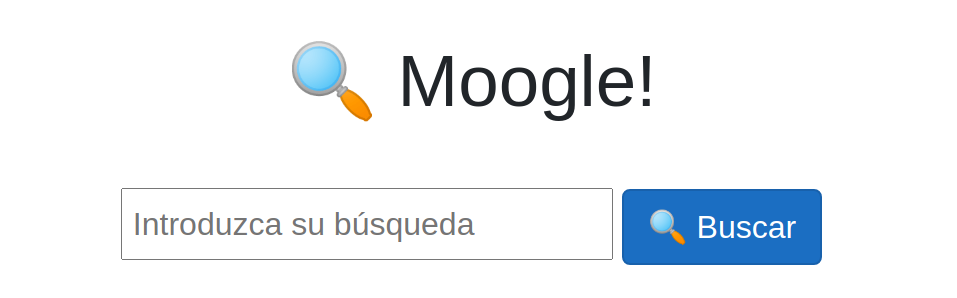
\includegraphics[width=15cm, height=4cm]{moogle.png}
\vfill
{\Large Leonardo Ojeda Hecheverria C-113 \par}
{\Large Curso 2023 \par}
\end{titlepage}
\pagestyle{headings}
\parskip 3em
\begin{center}
\end{center}
\begin{flushleft}
\begin{Huge}
Funcionamiento de MOOGLE!
\end{Huge}
\setcounter{secnumdepth}{1}
\section{•Descripción}

\end{flushleft}
\begin{Large}
Moogle! es un buscador local de texto que
utiliza el modelo vectorial TF-IDF para
obtener una mejora importante de eficacia y
rapidez. Se basa en la idea de crear una base
de datos con los documentos en los que se
quiere trabajar, evaluar la similaridad entre el
contenido de estos y la búsqueda realizada por
el usuario, ordenar los documentos por este
coeficiente y finalmente mostrarle en pantalla los
documentos coincidentes ordenados, más una
frase contenida en este donde puede
encontrarse su búsqueda o algo relacionado
con esta.

\end{Large}

\section{•Funcionalidad}
\begin{Large}

   
- El método GetDocuments():
Este método devuelve una lista de todos los 
documentos en una determinada ubicación de contenido.
Utiliza la clase Directory del espacio de 
nombres System.IO para obtener los nombres 
de archivo que coinciden con un patrón específico (*.txt) 
en la ruta de contenido especificada.
Retorna un array de cadenas que representa
los nombres de archivo de los documentos encontrados.

- El método GetTerms(string documentPath, bool document):
Este método toma la ruta de un documento y una 
bandera que indica si 
se debe leer el texto del archivo o si el
texto ya se ha proporcionado como argumento.
Usa el método ReadAllText() de la clase 
File para leer todo el texto de un archivo en una cadena.
Luego, divide la cadena en palabras utilizando
el método Split() y filtra las palabras vacías.
Después, se eliminan los caracteres de puntuación
y se convierten las palabras a minúsculas.
Retorna un array de cadenas que representa los 
términos del documento.

- El método GetTermFrequency(string term, 
string document, Dictionary<string, Dictionary
<string, int>> invertedIndex):
Este método toma un término, un documento y 
un índice invertido como argumentos. Verifica si 
el término existe en 
el índice invertido y si el documento tiene una 
frecuencia asociada al término.
Retorna la frecuencia del término en el documento o 
0 si no se encuentra.


- El método CreateInvertedIndex(string[] documents):
Este método toma un array de nombres de archivo de 
documentos como argumento.
Crea un índice invertido vacío representado por un diccionario.
Itera sobre cada documento y obtiene los 
términos utilizando el método GetTerms().
Luego, actualiza el índice invertido aumentando 
la frecuencia de aparición de cada término en cada documento.
Retorna el índice invertido completo.

- Estos métodos trabajan en conjunto para leer y procesar 
una consulta, así como para calcular la relevancia en cada 
documento utilizando un índice invertido.

- El metodo CalculateDocumentMagnitudes(Dictionary<string, 
Dictionary<string, int>> invertedIndex):
Este método calcula la magnitud de cada 
documento en función de su frecuencia de 
aparición en el índice invertido.
Itera sobre los documentos y por cada 
documento, itera sobre los postings en el índice invertido. 
Acumula la suma de los cuadrados de las 
frecuencias de cada documento.
Calcula la raíz cuadrada de la suma de los cuadrados, 
lo cual representa la magnitud del documento.
Almacena la magnitud de cada documento en un diccionario 
(documentMagnitudes), donde la clave es el nombre del 
documento y el valor es su magnitud. 

- El método CreateQueryVector(string query, Dictionary<string, 
Dictionary<string, int>> invertedIndex):
Este método crea un vector de consulta que mapea los términos
a sus pesos en base a su frecuencia y su IDF (Inverse Document Frequency).
Obtiene los términos de la consulta utilizando el método GetTerms.
Crea un diccionario llamado queryVector para almacenar 
los pesos de los términos de la consulta.
Calcula el peso de cada término en la consulta utilizando 
la fórmula tf-idf (term frequency-inverse document frequency).
Agrega cada término y su peso al diccionario queryVector.
Finalmente, retorna el diccionario queryVector que representa el vector de consulta.

- El método CalculateScore(string document, Dictionary<string, double> 
queryVector, Dictionary<string, Dictionary<string, int>> invertedIndex, 
Dictionary<string, double> documentMagnitudes):
Este método calcula el puntaje de similitud de un documento en 
base a su similitud coseno con la consulta, la ponderación de 
los términos de la consulta que se ajustan al documento y la 
rareza de los términos de la consulta.
Obtiene el número total de documentos en el índice invertido.
Itera sobre los términos y verifica si existen en el índice invertido.
Calcula la frecuencia del término en el documento y realiza 
ajustes adicionales según ciertas condiciones.
Calcula el peso del término en la consulta y en el documento 
utilizando la fórmula del puntaje coseno.
Realiza la normalización del puntaje del documento dividiéndolo 
por su magnitud, si está disponible.
Retorna el puntaje del documento.


\begin{displaymath}
SimCos(d_{(d)},q)=\frac{\displaystyle\sum_{n=1}(P_{(n,d)}\times P_{(n,q)})}{\sqrt{\displaystyle\sum_{n=1}(P_{(n,d)})^2 \times \displaystyle\sum_{n=1}(P_{(n,q)})^2}}
\end{displaymath}



\section{Ejecutando MOOGLE!}
Debe colocar los documentos en los que quiere desarrollar la búsqueda, en la carpeta
"Content", en formato ".txt".  

-Este proyecto está desarrollado para la versión objetivo de .NET Core 6.0. Para ejecutarlo debe ir a la ruta en la que está ubicada el proyecto y ejecutar en la terminal de Linux:

\begin{flushleft}
```bash\newline
make dev
```

- Si está en Windows, debe poder hacer lo mismo desde la terminal del WSL (Windows Subsystem for Linux), en caso contrario puede ejecutar:

```bash\newline
dotnet watch run --project MoogleServer
```

- También puede ejecutar el archivo Script.sh dentro de la carpeta Script y usar el comando "run".

\end{flushleft}
\section{•Consideraciones}
-Este programa ha sido desarrollado para
buscar en documentos en español, y no se
asegura su correcto funcionamiento en otro
idioma.\\
\newline
-La rapidez de este programa depende
necesariamente del número de documentos y
su tamaño. Su rendimiento se
verá necesariamente afectado para un número demasiado
grande de documentos extensos.
\end{Large}

\end{document}
